 \let\negmedspace\undefined
\let\negthickspace\undefined
\documentclass[journal]{IEEEtran}
\usepackage[a5paper, margin=10mm, onecolumn]{geometry}
\usepackage{lmodern} % Ensure lmodern is loaded for pdflatex
\usepackage{tfrupee} % Include tfrupee package

\setlength{\headheight}{1cm} % Set the height of the header box
\setlength{\headsep}{0mm}     % Set the distance between the header box and the top of the text

\usepackage{gvv-book}
\usepackage{gvv}
\usepackage{cite}
\usepackage{amsmath,amssymb,amsfonts,amsthm}
\usepackage{algorithmic}
\usepackage{graphicx}
\usepackage{textcomp}
\usepackage{xcolor}
\usepackage{txfonts}
\usepackage{listings}
\usepackage{enumitem}
\usepackage{mathtools}
\usepackage{gensymb}
\usepackage{comment}
\usepackage[breaklinks=true]{hyperref}
\usepackage{tkz-euclide} 
\usepackage{listings}
\usepackage{gvv}                                        
\def\inputGnumericTable{}                       
\usepackage[latin1]{inputenc}                                
\usepackage{color}                                            
\usepackage{array}                                            
\usepackage{longtable}                                       
\usepackage{calc}                                             
\usepackage{multirow}                                         
\usepackage{hhline}                                           
\usepackage{ifthen}                                           
\usepackage{lscape}  
\usetikzlibrary{patterns}
\begin{document}
\bibliographystyle{IEEEtran}


\textbf{Question 2.2.19:} \\
\textbf{} The scalar product of the vector $\hat{i} + \hat{j} + \hat{k}$ with a unit vector along the sum of vectors 
$2\hat{i} + 4\hat{j} - 5\hat{k} \quad \text{and} \quad \lambda \hat{i} + 2\hat{j} + 3\hat{k}$ is equal to one. Find the value of $\lambda$.


\textbf{Solution:}\\
 \textbf{Given}  
\begin{align}
\vec u = \myvec{1\\1\\1}, \quad 
\vec a = \myvec{2\\4\\-5}, \quad 
\vec b = \myvec{\lambda\\2\\3}
\end{align}
We require:  
\begin{align}
\vec u^\top \frac{\vec a+\vec b}{\|\vec a+\vec b\|} = 1
\end{align}

\textbf{Sum of vectors:}
\begin{align}
\vec a + \vec b = \myvec{2+\lambda\\6\\-2}
\end{align}

\textbf{Dot product:}
\begin{align}
\vec u^\top(\vec a+\vec b) = \myvec{1 & 1 & 1}\myvec{2+\lambda\\6\\-2} 
= (2+\lambda)+6+(-2) = \lambda+6
\end{align}

\textbf{Norm of the sum:}
\begin{align}
\|\vec a+\vec b\| = \sqrt{(2+\lambda)^2+6^2+(-2)^2}
= \sqrt{(2+\lambda)^2+40}
\end{align}

 \textbf{Condition:}
\begin{align}
\frac{\lambda+6}{\sqrt{(2+\lambda)^2+40}} = 1
\end{align}

\textbf{Simplify:}
\begin{align}
\lambda+6 = \sqrt{(\lambda+2)^2+40}
\end{align}
Squaring,
\begin{align}
(\lambda+6)^2 = (\lambda+2)^2+40
\end{align}
\begin{align}
\lambda^2+12\lambda+36 = \lambda^2+4\lambda+44
\end{align}
\begin{align}
8\lambda = 8 \quad \Rightarrow \quad \lambda = 1
\end{align}
\textbf{Conclusion:}  
The required value is
\begin{align}
\boxed{\lambda=1}
\end{align}
\begin{align}
\boxed{\,a = -3\,}
\end{align}
\newpage
\begin{figure}
    \centering
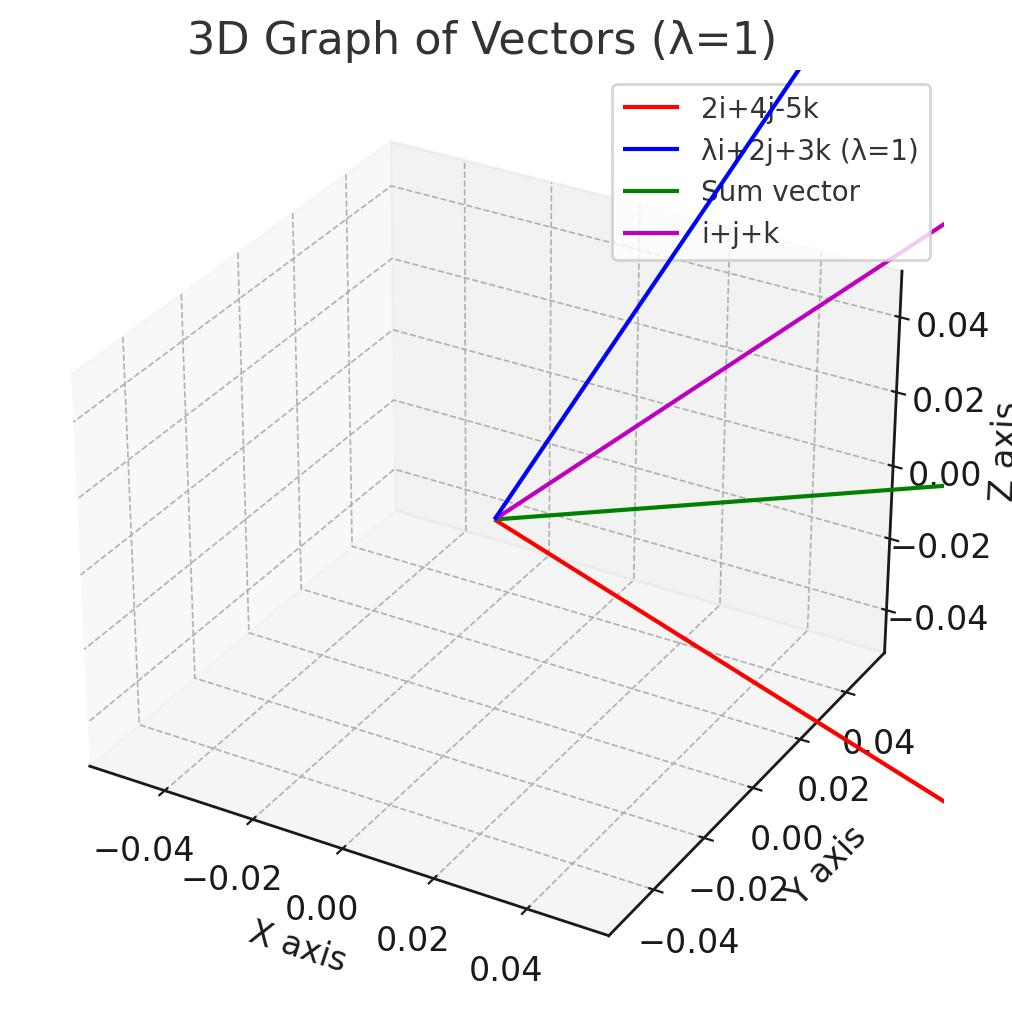
\includegraphics[width=0.5\linewidth]{beamer/figs/matg3.jpeg}
    \caption{}
    \label{fig:placeholder}
\end{figure}
\end{document}